\documentclass[10pt]{article}
\usepackage[letterpaper,margin=1in]{geometry}
\usepackage[T1]{fontenc}
\usepackage{amsmath,amsthm,mathtools}
\usepackage{newtxtext,newtxmath,microtype}
\usepackage[numbers,sort&compress]{natbib}
\usepackage{tikz,pgfplots,graphicx}
\usetikzlibrary{arrows.meta,positioning,calc}
\pgfplotsset{compat=1.18}
\usepackage{caption}
\captionsetup{font=small,skip=7pt}
\usepackage[hidelinks]{hyperref}
\usepackage{url}
\hypersetup{pdftitle={A reachable-state separation between attention compression and its certificates},pdfauthor={Samuel Mausberg}}
\widowpenalty=10000\clubpenalty=10000
\setlength{\parindent}{1em}\setlength{\parskip}{3pt}
\setlength{\emergencystretch}{1.6em}
\newtheorem{theorem}{Theorem}
\newtheorem{lemma}[theorem]{Lemma}
\newtheorem{corollary}[theorem]{Corollary}
\theoremstyle{definition}\newtheorem{definition}[theorem]{Definition}
\newcommand{\TV}{\operatorname{TV}}
\newcommand{\KL}{D_{\mathrm{KL}}}
\newcommand{\osc}{\operatorname{osc}}
\newcommand{\Lip}{\operatorname{Lip}}
\newcommand{\R}{\mathbb R}
\newcommand{\B}{\mathcal B}
\newcommand{\Pcal}{\mathcal P}
\newcommand{\E}{\mathbb E}
\newcommand{\TechAccept}{1019}
\newcommand{\LitAccept}{961}
\newcommand{\TechFallback}{5}
\newcommand{\LitFallback}{63}
\newcommand{\TechPrefill}{14.718}
\newcommand{\TechDecode}{186.853}
\newcommand{\TechTotal}{202.042}
\newcommand{\LitTotal}{267.006}
\newcommand{\TechRSS}{1555.5}
\newcommand{\PackingSeconds}{23.869}
\newcommand{\TechLower}{83.957}
\newcommand{\TechRef}{11.354}
\newcommand{\TechCand}{34.385}
\newcommand{\TechCheck}{50.743}
\newcommand{\TechBase}{164.573}
\newcommand{\LitBase}{184.962}

\title{A reachable-state separation between\newline attention compression and its certificates}
\author{Samuel Mausberg}
\date{4 October 2026}
\begin{document}
\maketitle
\begin{abstract}
Does a certificate's refusal reflect the model's sensitivity or information lost by the proof? At a 7,168-token prompt in frozen SmolLM2-135M, we find a separation between the two. First, the specified centroid/coordinate-box and scalar-envelope certificate still refuses tenfold grouping after replacing its global readout gain with a sound local enclosure. Exact packing witnesses require at least 28.88\% of dense final-layer interactions, even with optimal allocation between heads. Second, a concrete tenfold grouping has a checked one-intervention sequence total variation of $1.148\times10^{-5}$, and a probability-weighted checker permits repeated interventions with a 1,024-token sequence guarantee below $0.000924$. The passing checker evaluates the dense reference and is slower than dense decoding.
\end{abstract}

\section{What the refusal means}
On a frozen pretrained transformer, a norm-based attention certificate can reject compression whose complete generated-sequence law stays within budget. We establish this separation at the terminal attention boundary of SmolLM2-135M. A sound local readout enclosure greatly reduces the global gain obtained at the origin, yet the specified certificate still rejects every partition small enough to give tenfold grouping. An explicit partition has a much smaller, directly checked effect on the output law. A second checker, which evaluates the reference logits, authorizes repeated compression while controlling the law of all 1,024 generated tokens.

The two findings use the same weights and stored attention inputs. For the norm-based certificate, we lower-bound the certificate of \emph{every} sufficiently small partition, allowing query-dependent groups and unequal allocation between heads. For the successful intervention, we run a concrete partition through the remainder of the network and check the categorical law of its executed logits. This compares an unavoidable certificate charge with the actual distributional effect of compression.

Differentiating the RMS-normalized readout at the origin gives a lower bound of 3,500 on the global readout gain. The recorded hidden vector instead has Euclidean norm about 948.989. Rational checks on its stored bits give
\begin{equation}\label{eq:localintro}
             0.28\ \leq\ C_1^*(x)\ \leq\ 0.746,
\end{equation}
where $C_1^*(x)$ is the optimal logit-oscillation gain on the radius-one ball around that vector. This ball excludes the origin, so the global constant substantially overstates the relevant local gain.

The local replacement still forces rejection. Coordinate-box summaries charge groups for query-weighted key separation and value separation. Exact clique witnesses convert these charges into nine convex, decreasing lower bounds on the attention certificates. The tenfold budget is $\lfloor64{,}512/10\rfloor=6{,}451$ groups across the final layer. Even the best allocation of those groups forces a declared logit-oscillation bound above 0.03731, while the complete-sequence budget permits at most 0.004 for a single intervention. At least 18,633 groups are necessary for this certificate to stop rejecting.

The concrete compression sorts rows by their query scores, keeps the highest-scoring 256 rows as singletons, and splits the rest into 460 groups. Each head's 7,168 rows are represented in 716 groups. Its next-token law has checked total variation (TV) of approximately $1.148\times10^{-5}$ from the single-row-tail reference. When compression occurs once and dense computation resumes afterwards, the complete 1,024-token sequence has exactly the same TV.

This equality follows from the location of the intervention. The last layer writes its keys and values from the preceding layer's states, before reading attention. Changing the read leaves all persistent KV state unchanged on a common token history. We change all nine heads at this boundary while the preceding twenty-nine blocks remain dense.

Recent work already examines vacuous compression certificates and output-aware risk control~\citep{pricingrisk,riskkv}. Our contribution is the specific checked separation: an all-partitions refusal with a verified local readout gain, a concrete compression below the sequence budget, and a passing repeated-intervention check at a KV-preserving boundary. Section~\ref{sec:related} distinguishes the guarantees.

\section{The executable and the comparison}
\label{sec:executable}
The frozen checkpoint is the released Q8\_0 export of SmolLM2-135M-Instruct~\citep{smollm,smollmcard,ggufrelease}. Its published SHA-256 is matched before loading. Our reference holds the exporter's dequantized tensors fixed in binary32; it is not the original BF16 checkpoint. The model has thirty blocks, width 576, nine query heads, three KV heads, and head dimension 64. Its native context limit is 8,192 tokens. The two rollout prompts each contain 7,168 tokens, leaving room for 1,024 outputs. One is a technical research note retained as \texttt{data/prompt.txt} in the replay bundle; the other is the opening of Lewis Carroll's public-domain \emph{Alice's Adventures in Wonderland}~\citep{alice}. Both prompt texts and token arrays are retained. The experiments leave the weights unchanged.

The CPU executor uses PyTorch 2.10.0, four compute threads, adjacent-pair RoPE for the GGUF-permuted query and key rows, and dense scaled-dot-product attention. Generation uses temperature one and no top-$k$, top-$p$, or stopping rule; EOS is an ordinary symbol in the fixed-length output law. A binary32 logit vector $z$ defines the ideal conditional law $\operatorname{softmax}(z)$. Appendix~\ref{app:arithmetic} specifies the finite sampler and bounds its difference from that law.

Floating-point evaluation order is part of the executable. In the first-intervention experiment, the prompt is evaluated densely and its last attention output is passed through a single-row final feed-forward block and readout. Replaying that tail in isolation changes the categorical law by $8.617\times10^{-7}$ relative to the original batched tail. In the rollout executor, only the last query of the prompt's final attention layer is evaluated; future tokens use the same single-query path. We distinguish these reference executables throughout. The final query vectors used by the packing witness and by the first rollout step agree bitwise. PyTorch documents that batched and slice computations can differ numerically~\citep{pytorchnumerics}.

The numerical controls keep every weight tensor and every attention row. One casts Q, K, and V to BF16 at each dense attention call and returns the output to binary32 before the remaining operations. The other uses FP64 inside attention with the same binary32 return boundary. These controlled variants isolate attention arithmetic within this executor, including input rounding in the BF16 case.

Once the executor has produced finite logits, an independent checker can compare their categorical laws using their exact stored values. This comparison includes the effects of all upstream rounding without requiring a proof of the preceding matrix multiplications. It establishes statements about the executed logits; equivalence to another SmolLM2 implementation would require a separate check. The replay bundle retains the logits and numerical witnesses. Appendix~\ref{app:arithmetic} gives the enclosure algorithms and their trust boundary.

\section{The refusal away from the origin}
\subsection{A sound local readout enclosure}
Write the final readout as
\begin{equation}\label{eq:readout}
 R(x)=\frac{A x}{\sqrt{a(x)}},\qquad
 A=W\operatorname{diag}(\gamma),\qquad
 a(x)=\frac{\|x\|_2^2}{D}+\varepsilon_R,
\end{equation}
where $D=576$, $W$ is the vocabulary projection, and $\gamma$ is the final RMSNorm weight. We use logit oscillation, $\osc(v)=\max_i v_i-\min_i v_i$, because a common logit shift does not change softmax. Define $C_\rho^*(x)$ to be the smallest Lipschitz constant from Euclidean distance to oscillation for $R$ on the closed ball $B(x,\rho)$.

For a pair of vocabulary rows, let $b=A_i-A_j$, $s=\|x\|^2$, and $u=b^\top x$. The squared gradient norm of their logit difference is
\begin{equation}\label{eq:gradient}
 \left\|\nabla(R_i-R_j)(x)\right\|^2
 =\frac{a^2\|b\|^2-2au^2/D+u^2s/D^2}{a^3}.
\end{equation}
Every term on the right is rational for stored binary32 inputs. Rows 1 and 216 give a value exceeding $(7/25)^2$. A derivative at the centre of any positive-radius ball is a lower bound on its Lipschitz constant, so $C_\rho^*(x)\geq0.28$ for every $\rho>0$.

The upper bound is also local. Differentiating the normalized vector gives
\[
 J(x)=a^{-1/2}\left(I-\frac{xx^\top}{Da}\right).
\]
Its tangential eigenvalues are $a^{-1/2}$ and its radial eigenvalue is $\varepsilon_R a^{-3/2}$, so $\|J(x)\|_2\leq a^{-1/2}$. Consequently,
\begin{equation}\label{eq:ballupper}
 C_\rho^*(x)\leq
 \frac{2\max_i\|A_i\|_2}
 {\sqrt{(\max\{0,\|x\|_2-\rho\})^2/D+\varepsilon_R}}.
\end{equation}
Exact checks give $\|x\|\geq948$ and $\max_i\|A_i\|\leq962407/65536$. Substituting $\rho=1$ in~\eqref{eq:ballupper} and checking the squared inequality rationally gives $C_1^*(x)\leq373/500=0.746$. The entrywise enclosure is described in Appendix~\ref{app:arithmetic}.

The enclosure class uses continuous Euclidean balls around a reached binary32 state. Its derivative bound belongs to the real map~\eqref{eq:readout}; roundoff-aware extensions that enclose this map and add nonnegative rounding allowances inherit the refusal. Finite reachable sets, anisotropic uncertainty sets, and direct floating-point relational invariants lie outside this class.

\subsection{From a centroid bound to a packing constraint}
For one head, fix a query $q$ and stored rows $(k_i,v_i)$. A partition $\Pcal$ has group means $\bar k_g,\bar v_g$ and sizes $m_g$. Let
\[
 w_g=m_g e^{q^\top\bar k_g/8},\qquad
 \pi_g=\frac{w_g}{\sum_h w_h},\qquad
 \hat a=\sum_g\pi_g\bar v_g.
\]
The coordinate-box radius and the value radius are
\begin{align}
 r_g&=\frac18\sum_c|q_c|
 \max\{k^{\max}_{gc}-\bar k_{gc},\bar k_{gc}-k^{\min}_{gc}\},\\
 \rho_g&\geq\max_{i\in g}\|v_i-\bar v_g\|_2.
\end{align}
The centred value-aware certificate studied here is
\begin{equation}\label{eq:box}
 \B_q(\Pcal)=\sum_g\pi_g\left[
 (e^{r_g}-1)\rho_g+
 (e^{r_g}-1-r_g)\|\bar v_g-\hat a\|_2\right].
\end{equation}
It upper-bounds the real attention-output error; Appendix~\ref{app:centred} gives the derivation. We allow exact arithmetic for this certificate, which can only help its admission test.

Let $p_i$ be the dense attention probabilities and $P_g=\sum_{i\in g}p_i$. Jensen's inequality gives a centroid partition function no larger than the dense one. Bounding scores inside a group then yields $\pi_g\geq e^{-r_g}P_g$. Dropping the second, nonnegative term in~\eqref{eq:box} leaves
\begin{equation}\label{eq:masscharge}
 \B_q(\Pcal)\geq\sum_g P_g(1-e^{-r_g})\rho_g.
\end{equation}
Every separated group therefore incurs a probability-weighted charge.

Join two rows when
\[
 \frac18\sum_c|q_c||k_{ic}-k_{jc}|\geq\eta,
 \qquad \|v_i-v_j\|_\infty\geq\nu.
\]
A group containing such a pair has $r_g\geq\eta/2$ and $\rho_g\geq\nu/2$. Its charge in~\eqref{eq:masscharge} is therefore at least $c_{\eta,\nu}P_g$, where we use the rational relaxation
\begin{equation}\label{eq:charge}
 c_{\eta,\nu}=\frac{\eta\nu}{2(2+\eta)}
 \leq \frac\nu2(1-e^{-\eta/2}).
\end{equation}
The inequality follows from $e^t\geq1+t$.

\begin{theorem}[Weighted packing refusal]\label{thm:packing}
Suppose $S$ is a clique of size $s$ in this separation graph and $\ell_i\leq p_i$ are nonnegative certified attention-mass lower bounds for its vertices. Sort these bounds as $\ell_{(1)}\geq\cdots\geq\ell_{(s)}$. Every partition into at most $M$ groups satisfies
\begin{equation}\label{eq:packing}
 \B_q(\Pcal)\geq f(M):=
 c_{\eta,\nu}\sum_{j=M+1}^{s}\ell_{(j)},
\end{equation}
where $f(M)=0$ for $M\geq s$.
\end{theorem}
\begin{proof}
Call a group good when it contains no separated pair. It contains at most one clique vertex. At most $M$ clique vertices can therefore lie in good groups. All remaining clique vertices lie in charged groups, whose total mass is at least the sum of all but the $M$ largest certified clique masses. Apply~\eqref{eq:masscharge} and~\eqref{eq:charge}.
\end{proof}

All nine final-layer heads have checked cliques at $\eta=\nu=1/2$, so $c_{\eta,\nu}=1/20$. Their sizes range from 7,135 to 7,165. The checker verifies every pair in each proposed clique and encloses every attention score and exponential before forming a mass lower bound. Any verified clique suffices; the search need not find a largest one.

\subsection{An optimal allocation still fails}
Let $O$ be the final layer's output projection. The envelope class concatenates the head error balls, applies an operator norm for $O$, passes the incoming error through the final feed-forward residual with coefficient one, adds a nonnegative allowance for the feed-forward branch, and finally applies a readout Lipschitz constant. Unit-gain passage is a rule of this certificate class, not a lower bound on the local gain of the block or its composition with the readout. A local enclosure that exploits contraction across that block lies outside the refusal. The class's declared logit-oscillation bound $r_{\rm env}$ must satisfy
\begin{equation}\label{eq:composition}
 r_{\rm env}\ \geq\ C\,\|O\|_2
             \left(\sum_{h=1}^{9}\B_h(\Pcal_h)^2\right)^{1/2}.
\end{equation}
A stored integer vector $v$ gives an exact Rayleigh witness
$\|Ov\|^2/\|v\|^2\geq(1937/100)^2$, hence $\|O\|_2\geq19.37$. This linear gain applies on every neighbourhood. Equation~\eqref{eq:localintro} allows us to take the necessary lower gain $C=0.28$.

The usual sequence argument~\citep{hoeffding1963,cover2006} gives
\begin{equation}\label{eq:hoeffding}
 \KL(Q\|P)\leq\frac18\E_Q\sum_t r_t^2,
 \qquad
 \TV(P,Q)\leq\frac14\sqrt{\sup_{\text{histories}}\sum_t r_t^2}.
\end{equation}
Even granting this first query the whole $10^{-3}$ sequence-TV allowance requires $r_{\rm env}\leq0.004$. Within the stated class, we set the feed-forward branch allowance and inherited KV uncertainty to zero and allow free knowledge of the best partition. Restoring either nonnegative allowance can only increase the declared bound.

The allocation problem is small enough to solve exactly:
\begin{equation}\label{eq:allocation}
 V(M)=\min_{\substack{M_h\in\mathbb N_0\\\sum_h M_h\leq M}}
                         \sum_h f_h(M_h)^2.
\end{equation}
Each $f_h$ is a decreasing tail sum of sorted masses. Its square is discrete convex, so assigning each next group to the largest remaining marginal decrease is optimal. The implementation compares rational marginal decreases. A final discrete supporting-line check verifies the allocation independently of the heap order; Appendix~\ref{app:allocation} gives the proof.

At $M=\lfloor64{,}512/10\rfloor=6{,}451$, the optimal relaxed allocation is recorded in the artifact and gives
\[
 0.28(19.37)\sqrt{V(6451)}>0.03731>0.004.
\]
The first budget at which this lower bound ceases to reject is 18,633, or 28.883\% of the dense final-layer interaction count. Ceasing to reject is only a necessary condition for admission: the local certificate contains additional nonnegative terms. Figure~\ref{fig:packing} shows the entire relevant frontier.

\begin{figure}[t]
\centering
\begin{tikzpicture}
\begin{semilogyaxis}[width=.91\linewidth,height=5.4cm,xmin=5,xmax=30,ymin=.003,ymax=.12,
 xlabel={Groups as a percentage of dense final-layer interactions},
 ylabel={Lower bound on declared logit oscillation},
 grid=major,grid style={dotted},legend style={font=\small,at={(.98,.98)},anchor=north east},
 tick label style={font=\small},label style={font=\small}]
\addplot[thick] table[x=percent,y=osc] {figures/joint.dat};
\addlegendentry{Optimal allocation of checked packing bounds}
\addplot[dashed,thick,domain=5:30] {0.004};\addlegendentry{Whole sequence allowance for one query}
\addplot[densely dotted] coordinates {(10,.003) (10,.12)};
\addplot[only marks,mark=*,mark size=2pt] coordinates {(10,0.03731187167535965) (28.88299851190476,.004)};
\node[anchor=east,font=\small] at (axis cs:9.5,.085) {$10\times$ budget};
\end{semilogyaxis}
\end{tikzpicture}
\caption{The specified scalar envelope still refuses every tenfold partition. The curve uses gains of 0.28 for the readout and 19.37 for the output projection, with optimal allocation between nine heads. It lower-bounds the declared certificate, not the measured output error. The crossing at 18,633 groups is a necessary condition for admission.}
\label{fig:packing}
\end{figure}

\section{What the executed compression changes}
\label{sec:shift}
We test a concrete query-informed partition from the class covered by the refusal. For each head, we evaluate all binary64 query scores of the stored binary32 rows and sort them stably. We keep $b$ highest-scoring rows as singleton groups and split the rest into $716-b$ consecutive groups in score order, with sizes differing by at most one. Group keys and values are ordinary unweighted means. Multiplicity is included in the centroid softmax. The final attention vector is cast to binary32 and run through the unchanged output projection, feed-forward sublayer, final normalization, and vocabulary projection.

Preserving high scores matters more than merely having a small number of groups. With 716 groups in time order, the checked categorical TV is 0.02837. Sorting by score but keeping no leading singletons reduces it only to 0.01974. Keeping 64 singleton rows reduces it to $4.4935\times10^{-5}$; keeping 256 reduces it further to $1.1476\times10^{-5}$. Every variant represents every row, and all nine heads are changed together. The comparisons are direct checks of the laws defined by the executed logits.

The 256-singleton partition falls within the all-partitions refusal, yet its output shift is below budget. Score sorting keeps projected variation small while allowing substantial variation among key coordinates and values. Coordinate extrema discard cancellations in the projection, Euclidean envelopes discard directions through the network, and the oscillation bound gives rare vocabulary outcomes the same extremal role as common ones. The true error remains below~\eqref{eq:box}; the certificate loses information needed to show how small it is.

There is an exact way to extend this first-output comparison to a complete sequence. Apply the compression only at the first output, then use the dense reference for the remaining outputs. Both evaluators retain the same KV arrays after the modified read. Conditional on the same first token, they therefore have the same continuation kernel.

\begin{theorem}[One-read sequence identity]\label{thm:one}
Let $p$ and $q$ be first-token laws, and let $K_i$ be the common conditional law of the remaining $T-1$ tokens after first token $i$. Then
\[
 \TV\bigl(p(i)K_i(y),q(i)K_i(y)\bigr)=\TV(p,q).
\]
\end{theorem}
\begin{proof}
For each $i$, nonnegativity of $K_i$ gives
$\sum_y |p(i)K_i(y)-q(i)K_i(y)|=|p(i)-q(i)|\sum_y K_i(y)=|p(i)-q(i)|$.
Sum over $i$ and divide by two.
\end{proof}

The first-intervention laws therefore have the TVs displayed in Figure~\ref{fig:tv} for any $T$, including 1,024. For the 256-singleton partition, the ideal softmax TV lies in $[1.14762374,1.14762375]\times10^{-5}$. Appendix~\ref{app:arithmetic} gives the exact finite-sampler value.

\begin{figure}[t]
\centering
\begin{tikzpicture}
\begin{semilogxaxis}[width=.70\linewidth,height=5.6cm,xmin=3e-7,xmax=.08,
 xlabel={Checked first-token total variation},ytick={1,2,3,4,5,6},
 yticklabels={Time-order means,Score-order means,Score + 64 singletons,Score + 256 singletons,Dense BF16 attention,Dense FP64 attention},
 ymin=.5,ymax=6.5,y dir=reverse,grid=major,grid style={dotted},tick label style={font=\small},label style={font=\small}]
\addplot[only marks,mark=*,mark size=2.6pt] table[x=tv,y=row] {figures/tv.dat};
\addplot[dashed] coordinates {(.001,.5) (.001,6.5)};
\node[font=\small,anchor=center,rotate=90,fill=white,inner sep=1pt] at (axis cs:.0013,3.5) {$10^{-3}$ sequence target};
\end{semilogxaxis}
\end{tikzpicture}
\caption{Compression error and ordinary dense numerical variation on the same prompt. The four centroid interventions are compared with their common single-row-tail reference; their first-token TV equals their complete one-read-intervention sequence TV. Dense arithmetic controls are compared with batched FP32, and their first-token TV lower-bounds complete-sequence TV under any continuation. The rigorous numerical intervals are narrower than the plotting symbols.}
\label{fig:tv}
\end{figure}

The dense BF16-attention control differs from dense FP32 by a checked first-token TV of $0.0030194849894$. Marginalization cannot increase TV, so the complete-sequence distance is at least this large under any continuation. The $10^{-3}$ requirement is stricter than this dense numerical difference on the tested prompt. The FP64-attention control is much closer, at approximately $1.68447\times10^{-6}$. A compression budget must therefore name its numerical reference, even when both implementations retain exact dense attention.

\section{A passing check for repeated interventions}
\label{sec:gate}
To control repeated interventions, the closed-loop checker evaluates both dense and centroid final-attention paths at every output, including their unchanged tails. It accepts the candidate when an integer-checked KL bound passes and otherwise samples the dense reference. At context length $n$, the candidate uses 256 singleton rows and $\lfloor n/10\rfloor$ groups per head.

The check retains the probability-weighted spread of the actual logit error rather than just its maximum range. Let $p=\operatorname{softmax}(z)$, $q=\operatorname{softmax}(\hat z)$, $\Delta=z-\hat z$, and $r=\osc(\Delta)$. For any scalar $c$ and $r<1$,
\begin{equation}\label{eq:moment}
 \KL(q\|p)\leq
 \frac{\E_q[(\Delta-c)^2]}{2(1-r)}.
\end{equation}
To see this, centre at $\E_q\Delta$ and write
$\KL(q\|p)=\log\E_q e^{\Delta-\E_q\Delta}$. The centred variable has magnitude at most $r$. The exponential series bounds its remainder by $x^2/[2(1-r)]$, and its mean is zero. Use $\log(1+u)\leq u$ and
$\operatorname{Var}_q\Delta\leq\E_q[(\Delta-c)^2]$. 

The distinction is visible at the first intervention. Its logit range is about $7.16\times10^{-4}$, too large for an equal allocation of the range-only budget over 1,024 outputs. Its checked second-moment KL bound is only about $4.43\times10^{-10}$, which fits the gate's per-token allowance
\begin{equation}\label{eq:kappa}
                       \kappa=\frac1{600000000}.
\end{equation}
The outcomes carrying most of the range have little probability. Comparing the two executed logit vectors retains that information without a hidden-state Lipschitz approximation.

The gate encloses every term in~\eqref{eq:moment} for the executed logits and compares the resulting bound with~\eqref{eq:kappa} by an integer cross-product. Range, precision, and arithmetic guard failures select the dense path. Appendix~\ref{app:gate-arithmetic} gives the integer construction.

\begin{figure}[t]
\centering
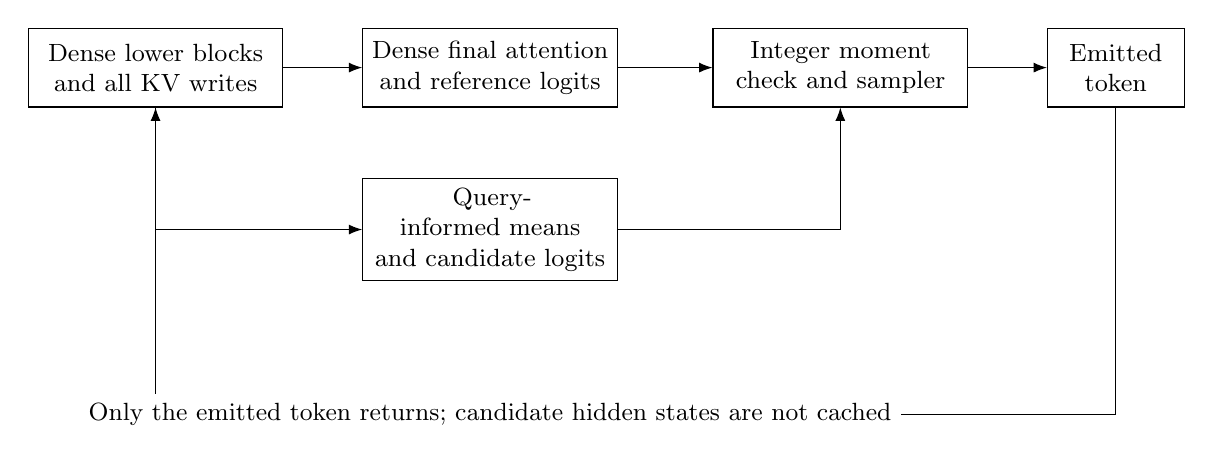
\begin{tikzpicture}[>=Latex,node distance=8mm,box/.style={draw,align=center,font=\small,minimum height=10mm,text width=30mm}]
\node[box] (lower) {Dense lower blocks\\and all KV writes};
\node[box,right=10mm of lower] (ref) {Dense final attention\\and reference logits};
\node[box,below=9mm of ref] (cand) {Query-informed means\\and candidate logits};
\node[box,right=12mm of ref,text width=30mm] (gate) {Integer moment\\check and sampler};
\node[box,right=10mm of gate,text width=15mm] (tok) {Emitted\\token};
\draw[->] (lower)--(ref);
\draw[->] (lower.south) |- (cand.west);
\draw[->] (ref)--(gate);
\draw[->] (cand.east)-|(gate.south);
\draw[->] (gate)--(tok);
\draw[->] (tok.south) |- ([yshift=-17mm]cand.south) -| (lower.south);
\node[font=\small,fill=white] at ([yshift=-17mm]cand.south) {Only the emitted token returns; candidate hidden states are not cached};
\end{tikzpicture}
\caption{The final read leaves persistent state unchanged. On a common token history, all KV entries are produced before the two attention branches, so the reference branch evaluates the dense model on that history. Token feedback follows the lower arrow. Timing includes both branches and the checker.}
\label{fig:boundary}
\end{figure}

\begin{samepage}
\begin{theorem}[Executable sequence bound]\label{thm:sequence}
Run the closed-loop terminal-attention gate for $T\leq1024$ outputs, accepting a candidate only when~\eqref{eq:moment} is certified to be at most $\kappa$. Suppose both evaluators use the finite sampler and its checked conditional-TV allowance $\delta_s$ from Appendix~\ref{app:sampler}. Write $P_{64}$ and $Q_{64}$ for their complete generated-sequence distributions, where the subscript denotes the sampler's 64-bit integer probability grid and uniform random word. Then
\begin{equation}\label{eq:programmetv}
 \TV(P_{64},Q_{64})
 \leq\sqrt{\frac{T\kappa}{2}}+2T\delta_s
 <0.000924.
\end{equation}
\end{theorem}
\begin{proof}
On every common token history, all KV entries are the same, since the changed read has no persistent output. The dense branch is therefore the conditional reference model on that history. The ideal-softmax hybrid has conditional KL at most $\kappa$ at an accepted step and zero at a rejected step. The autoregressive KL chain rule and Pinsker's inequality give $\TV(P,Q)\leq\sqrt{T\kappa/2}$. Coupling each finite sampler to its ideal conditional law gives $\TV(P_{64},P)\leq T\delta_s$ and $\TV(Q_{64},Q)\leq T\delta_s$. The triangle inequality gives~\eqref{eq:programmetv}. Its final strict numerical comparison is checked by squaring a positive rational residual.
\end{proof}
\end{samepage}

The guarantee holds over all histories of the gated program because every output must pass the same check or use dense fallback. The sampled executions below measure how often this rule accepts compression.

In the technical execution the gate accepts \TechAccept\ nonidentical candidate logit vectors and falls back at \TechFallback\ steps. Three fallbacks exceed the KL allowance and two trigger the conservative precision guard. In the Alice execution it accepts \LitAccept\ candidates and falls back at \LitFallback\ steps: four exceed the KL allowance and fifty-nine trigger precision guards. These counts describe two sampled continuations, not a workload-population acceptance rate. Figure~\ref{fig:trace} shows the checked conditional KL bounds that determine the decisions.

\begin{figure}[t]
\centering
\begin{tikzpicture}
\begin{semilogyaxis}[width=.92\linewidth,height=5.2cm,xmin=0,xmax=1024,ymin=1e-16,ymax=1e-7,
 xlabel={Generated-token index},ylabel={Candidate conditional KL upper bound},
 grid=major,grid style={dotted},legend columns=2,legend style={font=\small,at={(.5,1.03)},anchor=south,draw=none},
 tick label style={font=\small},label style={font=\small}]
\addplot[thin] table[x=step,y=kl] {figures/technical.dat};\addlegendentry{Technical prompt}
\addplot[thin,densely dotted] table[x=step,y=kl] {figures/alice.dat};\addlegendentry{Alice prompt}
\addplot[dashed,thick,domain=0:1024] {1/600000000};\addlegendentry{Admission cap}
\addplot[only marks,mark=x,mark size=2pt] table[x=step,y=kl] {figures/rejected.dat};\addlegendentry{KL-based dense fallback}
\end{semilogyaxis}
\end{tikzpicture}
\caption{Checked candidate KL bounds on two sampled continuations. Values above the cap cause dense fallback. Precision-guard failures have no computed KL bound and are omitted from the curves. The sequence guarantee follows from enforcing the cap at every history.}
\label{fig:trace}
\end{figure}

\section{The computation the passing proof costs}
\label{sec:cost}
The passing check scans every score, sorts the rows, reads all values to form means, and evaluates both dense final attention and the two logit tails. It retains the full raw cache. These operations make the query cost at least linear in context length. All of them are charged below.

On the four-thread AMD EPYC 9V74 CPU at concurrency one, the technical replay takes \TechPrefill\ seconds for prefill and \TechDecode\ seconds for its 1,024-output decode, or \TechTotal\ seconds including checkpoint load. Its measured decode phases include \TechLower\ seconds for the dense lower blocks and KV updates, \TechRef\ seconds for the reference terminal path, \TechCand\ seconds for centroid construction and the candidate terminal path, and \TechCheck\ seconds for the integer laws and checks. Sampling, logging, saved snapshots, and loop overhead account for the remainder. The Alice execution takes \LitTotal\ seconds including loading and prompt preparation.

The compatible dense control removes only the candidate branch and retains the reference executor and sampler. It takes \TechBase\ seconds end to end for the technical prompt and \LitBase\ seconds for the Alice prompt. The checked method is slower in both comparisons, so it cannot beat the fastest compatible implementation on this hardware. A positive performance comparison on supported GPUs would also need optimized exact attention such as FlashAttention-4~\citep{fa4}. Appendix~\ref{app:artifact} records the matched sampling protocol.

At 7,168 tokens, the binary32 raw KV payload is exactly 315 MiB; the allocated 8,192-token capacity is 360 MiB. The technical checked replay reaches a process peak of \TechRSS\ MiB, including weights, cache, prefill temporaries, and the checker. The separate packing audit takes \PackingSeconds\ seconds for the nine final heads and the local norm checks. That offline audit is separate from the rollout algorithm and its timings.

\section{Relation to prior work}
\label{sec:related}
Quest selects query-relevant pages, while Multipole Attention treats important rows exactly and approximates the rest through centroids~\citep{quest,multipole}. SPLA combines sparse and linear attention~\citep{spla}. Our partition uses these established representation ideas and full-score sorting to isolate their effect on the output law. The packing theorem concerns the certificate's charge for every partition in this class, rather than the computational hardness of attention studied by \citet{alman}.

Calver gives runtime per-head, per-step attention bounds with fallback~\citep{calver}. WitCert studies witness tightness, saturation, runtime gating, and cross-layer cancellation~\citep{witcert}. These works already distinguish soundness from usefulness. Local Lipschitz enclosures and the information-theoretic composition used here are also established tools~\citep{local,hoeffding1963,cover2006}.

\citet{pricingrisk} study adaptive admission for compressed serving state. Their mass-weighted logit moments imply expected conditional-output TV under compressor randomness, then an anytime tail bound on accumulated conditional losses. They also compare paired reference and compressed logits, finding that probability-weighted bounds can remain useful when worst-coordinate bounds are vacuous. Their witness-to-served-output audit also reports a 1,064-fold gap between the deployed witness threshold and the threshold needed by their sound per-read attention-TV law for a 5\% target; the query-norm envelope accounts for only a factor of 1.50~\citep[Section~7]{pricingrisk}. This is precedent for the separation phenomenon studied here, at the per-read attention tier. Our output-aware diagnosis builds on these observations. The difference is the checked all-partitions packing refusal with a non-origin local readout enclosure, paired with a concrete below-budget sequence law. At the KV-preserving final read, the integer gate enforces a conditional KL cap at every emitted history; this yields TV of the complete token sequence under the specified finite sampler. Their cumulative-loss tail bound and this sequence-law distance are different guarantees.

\citet{riskkv} use fixed-sequence Learn-then-Test to select KV-eviction policies. Calibration controls, with stated confidence, the population frequency of a task-utility drop exceeding a chosen tolerance. Their empirical-versus-certified comparisons already show that a policy can meet an observed risk target and still fail certification. Here the refusal is an exact lower bound for every sufficiently small partition, and the successful guarantee concerns the full token law for a fixed prompt. It requires no calibration population: the runtime checker evaluates every conditional decision. The intervention retains all KV entries and changes their final-layer read rather than evicting cache entries.

The contribution is therefore this finite-checkpoint separation and its executable repeated-intervention check, rather than the general use of output weighting or risk-controlled compression.

\section{Conclusion}
The measured terminal-attention boundary separates compression quality from the information retained by its certificate. Replacing the origin-based readout gain by a verified local enclosure still leaves an all-partitions refusal of tenfold grouping in the specified scalar-envelope class. A concrete partition has a small checked sequence shift, and a probability-weighted gate supports repeated interventions within the 1,024-token budget. The next computational question is how to obtain enough output-sensitive information for admission without evaluating the dense reference at every step.

\paragraph{Limitations.}
The separation is established on one frozen checkpoint at a KV-preserving final-layer boundary, with two sampled continuations. It leaves earlier-layer state compression and workload-population acceptance rates open. The refusal covers the stated coordinate-box and scalar Euclidean envelopes, while the passing checker trades dense reference computation for its guarantee. The precision controls compare variants of the supplied executor. Numerical checks trust the stated integer implementations. The Lean development checks only finite-kernel and shared-state identities and rational arithmetic.

\appendix
\section{Derivation of the centred attention certificate}
\label{app:centred}
Write $u_i=q^\top(k_i-\bar k_g)/8$ and $d_i=v_i-\bar v_g$ inside group $g$. Then $\sum_{i\in g}u_i=0$, $\sum_{i\in g}d_i=0$, $|u_i|\leq r_g$, and $\|d_i\|\leq\rho_g$. Let $\hat Z=\sum_gm_ge^{q^\top\bar k_g/8}$ and let $Z$ be the dense partition function. Jensen's inequality gives $Z\geq\hat Z$. Since $\sum_gw_g(\bar v_g-\hat a)=0$, the exact attention error can be written as
\begin{align*}
 a-\hat a
 &=\frac1Z\sum_g e^{q^\top\bar k_g/8}
 \left[\sum_{i\in g}(e^{u_i}-1)d_i
       +\sum_{i\in g}(e^{u_i}-1-u_i)(\bar v_g-\hat a)\right].
\end{align*}
Use $|e^{u_i}-1|\leq e^{r_g}-1$, $0\leq e^{u_i}-1-u_i\leq e^{r_g}-1-r_g$, and $Z\geq\hat Z$. The triangle inequality then gives~\eqref{eq:box}. Thus the second-order mass term is a consequence of centring the group, while the first term still pays for value variation.

For the lower bound, the group's dense unnormalized mass is at most $e^{r_g}w_g$. Therefore
$P_g\leq e^{r_g}w_g/Z\leq e^{r_g}w_g/\hat Z=e^{r_g}\pi_g$.
This proves~\eqref{eq:masscharge}. For two members of a group, coordinatewise triangle inequalities give
$\sum_c|q_c||k_{ic}-k_{jc}|/8\leq2r_g$, while the value triangle inequality gives $\|v_i-v_j\|_\infty\leq2\rho_g$. No assumption about a tree, contiguous pages, or a clustering heuristic enters these steps.

The means above are mathematical objects. A floating-point implementation can enclose its rounded means relative to these real means and add the corresponding nonnegative rounding terms. Such an extension inherits the refusal.

\section{Exact allocation across heads}
\label{app:allocation}
Fix one head and let $a_j=c\ell_{(j)}$ be its sorted nonnegative masses. Write $f(m)=\sum_{j>m}a_j$ and $F(m)=f(m)^2$. The gain from adding the next group is
\[
 D(m)=F(m)-F(m+1)=2f(m)a_{m+1}-a_{m+1}^2.
\]
It is nonnegative. If $a=a_{m+1}$, $b=a_{m+2}$, and $t=f(m+2)$, then
\[
 D(m)-D(m+1)=a^2+2ab-b^2+2t(a-b)\geq0,
\]
because $a\geq b\geq0$. Thus the available marginal decreases form a nonincreasing sequence in each head. Selecting the largest $M$ decreases respects their within-head order and minimizes the sum of the squared tails.

The checker also verifies a discrete dual certificate. At the proposed allocation $m_h$, choose a rational $\lambda$ no smaller than any next marginal decrease and no greater than any last selected decrease. Discrete convexity gives, for every alternative integer $u_h$,
\[
 F_h(u_h)\geq F_h(m_h)-\lambda(u_h-m_h).
\]
Summing this inequality proves optimality whenever $\sum_hu_h\leq\sum_hm_h$. The saved $\lambda$ and objective value are exact rationals. This supporting-line check verifies optimality independently of the allocation procedure.

For a cheaper headwise refusal, the final head with index 5 has a checked lower certificate charge above $0.00861$ at 716 groups. Its output-projection block has a rationally checked norm lower bound of 3. Together with the local readout lower bound 0.28, this already forces a declared range above $0.00723$, exceeding the whole single-query allowance 0.004. The joint argument is stronger because it permits unequal head budgets and uses the full projection's checked norm.

\section{Arithmetic, probability laws, and implementation guards}
\label{app:arithmetic}
\subsection{Readout and packing enclosures}
For the readout upper bound, the checker rounds every absolute weighted-row entry upwards on a $2^{-16}$ grid. Integer squared sums give $\max_i\|A_i\|\leq962407/65536$. Together with the exact check $\|x\|\geq948$, these bounds yield $C_1^*(x)\leq373/500=0.746$ by rational comparison of squared quantities.

The packing checker regards every stored binary32 entry as an exact dyadic rational. Keys and values are floored onto a $2^{-10}$ grid. If two integer coordinates differ by $b$, then $\max\{b-1,0\}/2^{10}$ is a conservative lower separation for their original coordinates. Query magnitudes are rounded down before forming the weighted key separation. Integer range guards are evaluated with Python integers before entering the fixed-width C++ pair checker.

Attention-mass bounds use a separate $2^{-20}$ grid to enclose each dot product. The common shift is an upper score bound, so all exponential arguments are nonpositive. An alternating Taylor series encloses $e^{-1/1024}$ by rationals; outward-rounded fixed-point squaring then encloses each required power. Normalizing an exponential lower numerator by the sum of exponential upper numerators gives the certified $\ell_i$. All divisions used in a refusal are rational cross-multiplications. The exact readout derivative, projection-vector witness, and discrete allocation comparisons use arbitrary-precision rational arithmetic.

\subsection{Categorical laws and the finite sampler}
\label{app:sampler}
For a saved logit vector, the independent checker finds a dyadic grid on which every logit is represented exactly. Taylor bounds on the grid's base exponential and 256-bit fixed-point exponentiation give per-coordinate exponential intervals. From $L_i\leq e_i\leq U_i$, it obtains
\[
 \frac{L_i}{Z_U}\leq p_i\leq\frac{U_i}{Z_L},\qquad
 Z_L=\sum_iL_i,\quad Z_U=\sum_iU_i.
\]
The TV upper bound is one minus the sum of lower overlaps. A fixed event selected from the approximate probability ordering gives a lower bound by subtracting its upper probability under one law from its lower probability under the other. Selecting an event numerically cannot invalidate that subsequent exact event check.

For the 256-singleton first intervention, the stored categorical counts give the sequence TV exactly as
\begin{equation}\label{eq:exacttv}
       \frac{211699215287897}{18446744073709551616}.
\end{equation}
For this count law, all non-pivot probability floors at denominator $2^{64}$ are resolved from these intervals. Remaining count mass is assigned to a maximum-logit pivot. The TV is then exactly half the integer $\ell_1$ count distance divided by $2^{64}$. The ideal softmax and this law differ by at most $(V-1)/2^{64}$, where $V=49152$.

The rollout uses a faster 96-bit C++ enclosure, with 256-bit intermediate products. It defines $q_i^L=L_i/Z_L$, floors its non-pivot probabilities at denominator $2^{64}$, and assigns the remainder to the pivot. Its deviation from ideal softmax is at most
\begin{equation}\label{eq:sampler}
 \frac{Z_U-Z_L}{Z_L}+\frac{V-1}{2^{64}}.
\end{equation}
Indeed, the true exponential vector is the lower vector plus a nonnegative residual, so its normalized law is a mixture of $q^L$ and the normalized residual. The first term bounds the mixture mass; the second bounds the probability floors. The runtime enforces $(Z_U-Z_L)/Z_L\leq10^{-12}$, giving the conditional-TV allowance used in Theorem~\ref{thm:sequence}:
\[
 \delta_s=10^{-12}+\frac{49151}{2^{64}}.
\]
 If the fast path's precision or range guard fails, the candidate is rejected and the high-precision reference sampler remains available. If a non-pivot probability floor remains unresolved after increasing precision, that sampler uses the lower-exponential law and the same checked width allowance instead of leaving the program undefined. This last branch was added during the implementation audit and was not needed in any recorded execution.

\subsection{Integer gate and guards}
\label{app:gate-arithmetic}
The binary32 logit difference is represented on a common dyadic grid. A dyadic centre $c$ is proposed near its numerically computed mean; any centre is valid in~\eqref{eq:moment}. The candidate's unnormalized exponentials are enclosed as integers $L_i\leq 2^{96}e^{\hat z_i-\max\hat z}\leq U_i$. With $Z_L=\sum_iL_i$,
\[
 \E_q[(\Delta-c)^2]
 \leq \frac{\sum_i U_i(\Delta_i-c)^2}{Z_L}.
\]
The gate compares the resulting KL bound with~\eqref{eq:kappa} by an integer cross-product. Failed range, precision, or arithmetic guards select the dense path.

With a common logit-error denominator $D_\Delta=2^b$, write $\Delta_i-c=d_i/D_\Delta$ and $r=R/D_\Delta$. The integer KL upper bound used by the gate is
\[
 \frac{\sum_i U_i d_i^2}{2Z_LD_\Delta(D_\Delta-R)}.
\]
The implementation checks $R<D_\Delta$ before forming a positive denominator. It bounds the vocabulary size, dyadic exponent, and signed differences before multiplication; the resulting numerator, denominator, and budget cross-products fit in 256 bits. A floating-point mean is used only to propose the integer centre. It has no trusted role in the inequality.

\subsection{Sampling assumptions and numerical trust}
Sampling draws a uniform 64-bit word and locates it in the arbitrary-precision cumulative integer counts. The proof assumes independent uniform words, as does the specification of a categorical sampler; the experiment records the operating-system-generated words for replay. The finite reference program maps any nonfinite logit vector to zero logits, and the hybrid uses the same totalization. No such case occurred in the recorded runs. This convention avoids leaving the program's probability law undefined on an untested history.

The integer operations, guards, and witness formats of the C++ and Python checkers form the trusted numerical implementation. Independent checks are included in the replay bundle. Its partial Lean development contains six declarations, checked with Lean 4.34.1 and the pinned Mathlib revision, with no \texttt{sorryAx} dependencies. These establish a finite-kernel $L^1$ identity, a shared-state identity, and rational arithmetic facts; \texttt{formal/check\_status.json} records their scope and axiom dependencies. The analytic inequalities, full KL chain rule, packing geometry and allocation theorem, numerical checker implementations, and transformer executor remain outside the formalized development.

\section{Reproduction and recorded execution}
\label{app:artifact}
The paper, source, and replay bundle are available in the \href{https://github.com/SamMausberg/attention-reachable-public-replay}{public replay repository}. The repository includes the retained witnesses, checker implementations, and reproduction instructions. The checkpoint is fetched separately from the release in~\citet{ggufrelease}; its SHA-256 is verified before tensor loading. The required digest is
\begin{center}\small\ttfamily
5a1395716f7913741cc51d98581b9b1228d8\allowbreak
0987a9f7d3664106742eb06bba83
\end{center}
The replay bundle contains both prompt-token arrays, the final-layer snapshot, nine clique witnesses, the reached-state and projection witnesses, exact categorical count laws for the first-intervention experiment, eleven paired snapshots from each rollout, complete token and random-word traces, raw timing records, and the figure-generation script. Full-vocabulary tensors used for the upper bound are reconstructed from the checkpoint.

The second prompt begins at Chapter~I of \emph{Alice's Adventures in Wonderland}, using the Project Gutenberg text~\citep{alice}, and is truncated to exactly 7,168 tokens without a chat wrapper or added beginning-of-sequence token. The retained UTF-8 excerpt fixes the whitespace; re-encoding it with the checkpoint tokenizer reproduces the saved token array. Its source, text and token digests, and selection record accompany the replay. The bundle retains the Alice execution and its dense control alongside the technical execution and the first-intervention and packing witnesses.

The compact replay checks the local readout lower bound, the projection witness, all clique separations, exact mass charges, the allocation refusal, and the rational sequence-budget comparison. A separate independent replay checks the saved categorical laws and paired logit witnesses. Verifying the all-vocabulary row-norm upper bound additionally requires the checkpoint, because it refers to every vocabulary row rather than only the witness pair. The complete executor and extraction scripts are included for that reproduction.

The recorded runs include checkpoint loading, prompt preparation, prefill, raw cache allocation and updates, sorting, centroid construction, dense fallback, integer probability construction, sampling, and trace output. The 28.883\% interaction floor concerns the final layer under the local readout bound; it does not bound the fraction of interactions required across all thirty layers.

The technical execution was replayed using its recorded 64-bit random words after replacing the sampler's vectorized cumulative sum with an arbitrary-precision cumulative sum. All 1,024 output tokens agree. Eleven saved technical logit pairs were independently checked with a 256-bit Python exponential enclosure; each upper second moment lies below the fast C++ enclosure. The same comparison was repeated for the ten Alice snapshots with a computed KL bound. The remaining Alice snapshot triggers a precision guard, and its served count law was checked against the reference fallback. Token-level TVs summarized from the sampled traces are numerical diagnostics rather than estimates of full-sequence TV.

The dense timing controls use the same reference executor, integer sampler, and recorded random words. The technical dense run first differs in emitted tokens at zero-based index 115. Shared-word inverse-CDF sampling is not a maximal coupling, so this mismatch gives no lower bound on the TV of the two laws. The two prompt experiments were not preregistered; the uniform program guarantee follows from the gate independently of their admission counts.

\section*{Acknowledgment of computational assistance}
The mathematical development, implementation, experiments, and manuscript revision were prepared with GPT-6 Astra Pro (OpenAI). The released records distinguish exact arithmetic checks, executed floating-point measurements, and the scope of the partial Lean development.

\bibliographystyle{plainnat}
\bibliography{references}
\end{document}
